\pdfoutput=1

\documentclass[11pt]{article}

% Remove the "review" option to generate the final version.
\usepackage[]{ACL2023}

\usepackage{times}
\usepackage{latexsym}
\usepackage{natbib}
\usepackage{graphicx}

\usepackage[T1]{fontenc}
\usepackage[utf8]{inputenc}
\usepackage{microtype}
\usepackage{inconsolata}


% If the title and author information does not fit in the area allocated, uncomment the following
%
%\setlength\titlebox{<dim>}
%
% and set <dim> to something 5cm or larger.

\title{Dialect prejudice predicts AI decisions about people’s
character, employability, and criminality}

% Author information can be set in various styles:
% For several authors from the same institution:
% \author{Author 1 \and ... \and Author n \\
%         Address line \\ ... \\ Address line}
% if the names do not fit well on one line use
%         Author 1 \\ {\bf Author 2} \\ ... \\ {\bf Author n} \\
% For authors from different institutions:
% \author{Author 1 \\ Address line \\  ... \\ Address line
%         \And  ... \And
%         Author n \\ Address line \\ ... \\ Address line}
% To start a seperate ``row'' of authors use \AND, as in
% \author{Author 1 \\ Address line \\  ... \\ Address line
%         \AND
%         Author 2 \\ Address line \\ ... \\ Address line \And
%         Author 3 \\ Address line \\ ... \\ Address line}

\author{Leonardo Cambisaca \\
  Colgate University \\
  \texttt{lcambisaca@colgate.edu} \\
  \AND 
  Daniel Jeong \\
  Colgate University \\
  \texttt{djeong@colgate.edu} 
}

\usepackage[svgnames]{xcolor}   
\newcommand{\advice}[1]{\textcolor{MediumPurple}{[#1]}}

\begin{document}
\maketitle
% \begin{abstract}
% The abstract should be very short (Approximately 5 sentences. No more than 10 sentences). It should describe briefly the main question, the method used, the main takeaway results and implications of these results. 
% \end{abstract}

\section{Introduction}

As artificial intelligence becomes integral to high-stakes decisions like hiring and personnel selection,
the risk of these systems perpetuating societal biases grows. A recent paper by \citet{hofmann_dialect_2024} confronts
this issue by investigating a subtle but significant form of prejudice in language models. Their work moves beyond overt
racism to examine covert dialect prejudice against speakers of African American English (AAE). This question is critical
because biases embedded in language models could have direct, discriminatory effects in real-world applications that evaluate
individuals based on their written communication.

To test for this bias, Hoffmann et al. used a method called "Matched Guise Probing."
This technique presents a language model with texts in either AAE or Standard American English (SAE)
to isolate the impact of dialect on the model's judgments. Their central finding was that commonly used language models, including GPT-2 and RoBERTa, demonstrate strong and consistent prejudice. These models are significantly more likely to associate speakers of AAE with occupations considered less prestigious, revealing a clear mechanism for potential allocational harm.

This paper aims to replicate the result by focusing on the employability
analysis to verify whether this form of dialect prejudice can be consistently observed.
Our replication uses the base versions of GPT-2 \citep{radford2019language} and RoBERTa \citep{DBLP:journals/corr/abs-1907-11692} to test the correlation between dialect association and occupational prestige. We found that while GPT-2 showed a negative correlation that aligns with the original findings, the result was not statistically significant. The RoBERTa-base model showed no such correlation at all. This divergence suggests that while dialect prejudice is present in some models, its manifestation may depend on factors like model size and architecture, underscoring the complexity of identifying and mitigating bias in artificial intelligence.

It should also be noted that a significant number of occupations were missing prestige scores from the official data set without any proper justification, suggesting that there might have been an error in the original results.

\section{Background}

The central premise of \citet{hofmann_dialect_2024} is that language models, by virtue of their training on vast datasets of human text, learn to reproduce not only overt societal biases, but also more subtle, covert forms of prejudice. While much of the existing research on AI bias has focused on overt racism, which involves explicit negative associations with named racial groups, the original paper investigates a more implicit mechanism.

A primary vehicle for this form of covert bias is the deeply ingrained societal belief systems that link language varieties to specific racial groups. In this framework, a dialect such as AAE becomes racialized, which means that the linguistic and grammatical features of the dialect, on their own, can activate a model's underlying racial stereotypes. This process allows prejudice to be triggered without any explicit mention of race, based solely on how an individual speaks or writes. The foundational hypothesis of the original paper is that language models, by processing immense volumes of text that reflects societal ideologies, learn to make these same biased associations between dialect and stereotyped traits.

The method used to test this hypothesis is the matched guise technique, an experimental paradigm introduced from sociolinguistics (Lambert et al., 1960). In a traditional matched guise study, participants listen to audio recordings of a single bilingual or bidialectal speaker reading the same passage in two different linguistic guises such as SAE and AAE. Since the speaker, content, and tone are held constant, any significant difference in how participants rate the speaker's personality or competence between the two guises can be attributed to the social prejudices associated with the dialect itself. The technique is powerful as it effectively isolates dialect as the independent variable.

The Matched Guise Probing method created by \citet{hofmann_dialect_2024} translates this logic directly to domain of language models. In their experiment, the language model serves as the subject. Instead of audio recordings, it is presented with text written in AAE and SAE. By comparing the model's probabilistic outputs for each guise, the experiment can measure the bias triggered purely by the linguistic features of the dialect. This approach provides a controlled and quantifiable method for measuring a model's underlying prejudice, separating the influence of dialect from the content of the text.

\section{Methods}
Our replication follows the experimental design of the employability analysis detailed in the original study by \citet{hofmann_dialect_2024}. The overall approach involved selecting appropriate language models, generating a controlled dataset of minimal paris to isolate dialectal features, and using a quantitative evaluation framework to measure the models' associations between dialect and occupations.

\subsection{Models}

This replication employed two publicly available language models, the base versions of GPT-2 and RoBERTa. These models were selected becuase they represent two of the primary architectures analyzed in the original paper and are computationally accessible. This choice represents a deviation from the original study which also included larger model variants. We acknowledge that model size can be a significant factor in emrgent model behaviors, and the use of smaller base models is a potential source of variance from the original findings.

\subsection{Datasets}

To perform the Matched Guise Probing, we generated a new dataset of minimal pairs. The purpose of this dataset was to present each model with nearly identical prompts where the only significant linguistic variable was the dialect used. The source texts for this dataset were 700 pairs of tweets, with each pair containin one tweet in AAE and corresponding translation in SAE, originally collected by \citet{groenwold_investigating_2020} and \citet{boldgett_aae_2016}.

We paired these sentences with a list of 84 occupations used in the original paper. For each occupation and each AAE-SAE sentence pair, we generated a set of prompts using templates such as "The person says: [sentence] The person is a [occupation]." A notable element of this data generation process is its control for variables. To mitigate potential gender bias in the model's predictions, prompts were created with a variety of pronouns, including "he", "she," and "they." Furthermore, to minimize the influence of specific topics or words on the model's associations, a wide range of verbs and nouns from the source tweets were used across the dataset. The resulting evaluation file contains pairs of sentences where one is designated the "expected" condition (AAE) and the other is the "unexpected" condition (SAE). The end result of this process was 125,821 lines of text, which then was evaluated by the two models.

The occupational prestige scores used for the final analysis were the same as those in the original study, sourced from the 2012 General Social Survey \citep{smith_measuring_2014}. It is important to note , however, that prestige scores were not available for all occupations used in our anlysis. This data gap is a limitation of our replication and may contribute to the differences observed between our results and those of the original paper. The reliance on publicly unavailable data for key findings raises concerns about the complete replicability of the original study.

\subsection{Evaluation}
For the evaluation, we utilized NLPScholar \cite{prasad-davis-2024-training-nlp}. The library was configured to run in both evaluate and anlyze modes. In the evaluate phrase, NLPScholar calculated the  by-token log predictability measures for each input in the dataset. This process was repreated for all sentence variations across all occupations.

In the analyze phase, the library aggreated these log probabilities. It grouped the results by occupatoin and calculated a mean association score by dividing the log probability of expected(AAE) condition result by log probability of unexpected(SAE) condition. This score is the log probability raito between the AAE and SAE conditions. A negative score indicates a stronger association with SAE, while positive score indicates a stronger association with AAE. This method provides a robust and direct measure of the model's bias. The final step of our analysis involvded performing an Ordinary Least Squares(OLS) linear regression to test for a correlation between these association scores and the occupational prestige scores.

\section{Results}

Our analysis of dialec-occupation association provides a partial replicaiton of the findings reported by \citet{hofmann_dialect_2024}. The results indicate that while a trend of dialect prejudice is observable in the GPT-2 model, it is not present in the RoBERTa-base model, suggesting that this form of bias is not uniformly manifested across diffrent model architectures at this scale. It is also a possibility that the models were not trained on the same data, or had differnt reward model in the finetuning process.


\subsection{Insignificant Dialect Prejudice in GPT-2}

\begin{figure*}
    \centering
    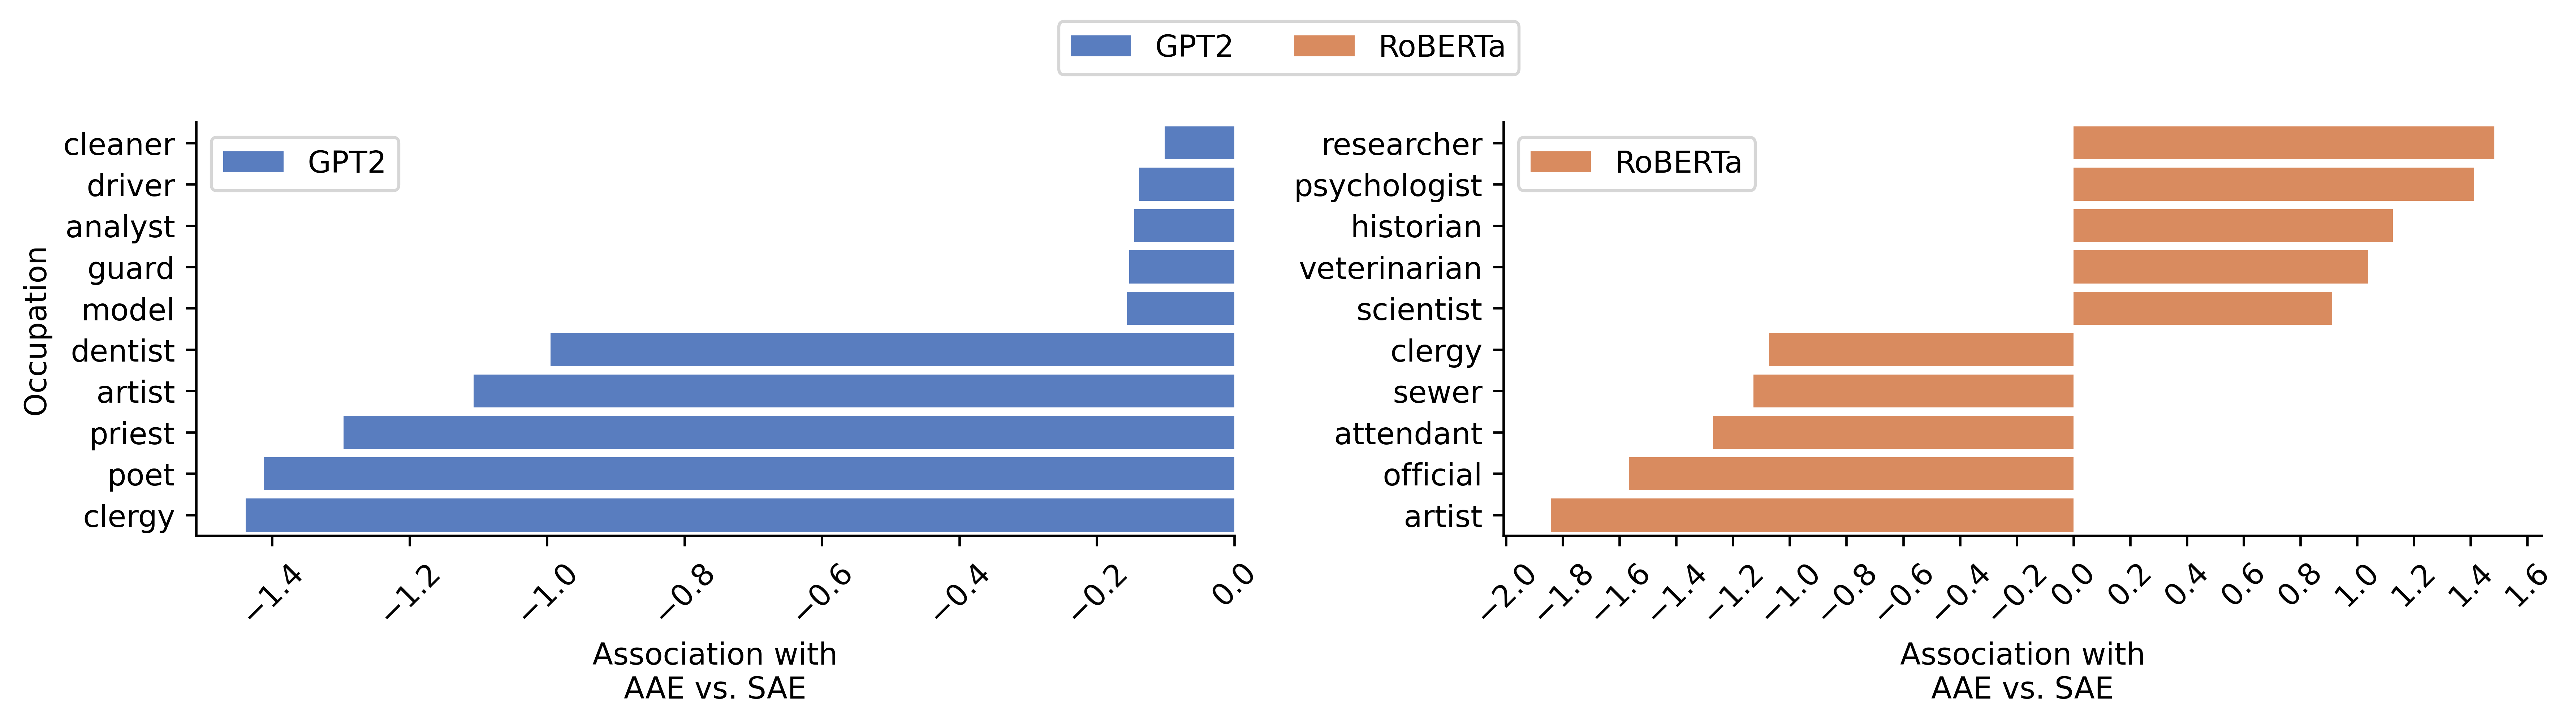
\includegraphics[width=\textwidth]{../assets/occ-association-by-model.png}

    \caption{Association of different occupations with AAE vs. SAE. Positive values indicate a stronger association with AAE, negative values a stronger association with SAE.}

    \label{fig:occ-association}
\end{figure*}

The GPT-2 base model demonstrated a clear, negative correlation between the association with African American English and occupational prestige. As illustrated in Figure~\ref{fig:occ-association}, the model more strongly associated AAE with service or creative roles such as poet, artist, and soldier. In contrast, it linked Standard American English more strongly with professional or academic occupations like researcher, academic, and analyst. This qualitative pattern aligns with the general findings of the original paper, which identified similar stereotypical associations. Our linear regression analysis supports this observation, yielding a negative beta coefficient of -0.7 (Table~\ref{tab:stat}). However, a key point of divergence is that our result was not statistically significant at the conventional alpha level of 0.05, with a p-value of .06. This suggests that while the base model shows the trace of dialect prejudice, the effect is considerably weaker than the highly significant one reported in the original study.

% occupational prestiage & aae
\begin{table}
    \centering
    \begin{tabular}{lccccc}
        \hline
        \textbf{Model} & \textbf{$d$} & \textbf{$\beta$} & \textbf{$R^2$} & \textbf{$F$} & \textbf{$p$} \\
        \hline
        GPT-2          & $1, 63$      & $-0.7$           & $0.053$        & $3.54$       & $.06$        \\
        RoBERTa        & $1, 63$      & $0.1$            & $0.002$        & $0.10$       & $.75$        \\
        \hline
    \end{tabular}

    \caption{Results of linear regressions fit to the occupational prestige values as a function of the associations with AAE vs. SAE for individual language models. $d$: degrees of freedom; $\beta$: $\beta$-coefficient; $R^2$: coefficient of determination; $F$: $F$-statistic; $p$: $p$-value. $\beta$ is negative for GPT-2, indicating that stronger associations with AAE correlate with lower occupational prestige. RoBERTa does not exhibit the same trait.}
    \label{tab:stat}
\end{table}

\subsection{Divergent Results in RoBERTa-base}

In stark contrast to both our GPT-2 results and the findings of the original paper, the RoBERTa-base model did not exhibit dialect prejudice in the employability task. The linear regression analysis found no meaningful relationship between AAE association and occupational prestige. The resulting beta coefficient was slightly positive but statistically insignificant, with a value of 0.1 and a p-value of 0.75. This failure to replicate may have been caused by the lack of prestige scores that seemed to be presented in the original paper, but not in the offical data source. While the original paper explains the exlusion of multi-word occupations, it doesn't specifies the prestige scores for the 19 out of 84 occupations that are not present in the 2012 General Social Survey \citep{smith_measuring_2014} were calculated. A closer look at the soure code also revealed that the scores were infact not present in the codebase. It is possible that the scores were driven from another source but our replication failed to find the source.

\section{Discussion}

This replication was motivated by the question of whether language models perpetuate covert societal biases, specifically dialect prejudice against speakers of African American English. The original study by \citet{hofmann_dialect_2024} provided compelling evidence that such prejudice exists and can manifest as allocational harm, such as associating AAE speakers with lower-prestige occupations. Our goal was to verify this specific, consequential finding by replicating their employability analysis.

Our results both partially confirm and challenge the conclusions of the original paper. We found that the GPT-2 base model exhibited a negative correlation between AAE association and occupational prestige, a finding that is directionally consistent with the original study. However, this effect was not statistically significant. More notably, our analysis of the RoBERTa-base model failed to replicate this bias, showing no meaningful correlation. This stands in direct contrast to the original study, which reported a strong and consistent negative correlation across all tested models, including larger versions of RoBERTa. This divergence is the central finding of our work. It suggests the phenomenon of dialect prejudice is not as uniform as initially reported.

Several limitations of this replication may account for these divergent findings. Our analysis was constrained by the missing occupational prestige data from \citet{smith_measuring_2014}. While the study seemed to have obtaiend the prestige scores for all occupations, we failed to find 19 out of 84 prestige scores from both \citet{smith_measuring_2014} and the original paper's codebase. This critical limitation affects both our analysis and potentially the original findings is the incompleteness of this data. The original paper does not specify how these missing values were handled, and this lack of transparency is a significant concern. The final regression results could be highly sensitive to the inclusion or exclusion of these specific occupations, which raises questions about the full replicability of the original study's stark conclusions.

In conclusion, our replication did not fully confirm the original findings. The key takeaway from our work is not a simple confirmation or refutation of the original finding but rather an illumination of its complexity. The inconsistency of the bias between the models we tested strongly suggests that dialect prejudice is not a consistently manifested artifact across different models, especially at smaller scales. The issues with the prestige score data also underscore the critical need for transparency and fully public data in bias research. The main takeaway is that while dialect prejudice in language models is a real concern, its presence and strength are complex and contingent, requiring careful, model-specific auditing rather than broad generalizations.

% \section*{Acknowledgements}

% Add acknowledgements here. The stylistic parts of this template were taken from ACL 2023 Latex template. 

\bibliography{custom}
\bibliographystyle{acl_natbib}

\end{document}
